\RequirePackage{xr}
\externaldocument{SARTexture-IT.R1}

\documentclass[journal,onecolumn,draftcls,11pt]{IEEEtran}

\usepackage{graphicx}
\usepackage{subfigure}
\usepackage{booktabs}
\usepackage[T1]{fontenc}
\usepackage[cmex10]{amsmath}
\usepackage{amsfonts}
\usepackage{color}
\usepackage{bm,bbm}
\usepackage{wasysym}
\usepackage{texnames}
\usepackage{todonotes}
\usepackage{url}
\usepackage[boxed]{algorithm2e}   % AAB inserido
\usepackage[listings]{tcolorbox}
\usepackage[binary-units]{siunitx}
\usepackage{multirow,bigstrut}
\usepackage{capt-of}
\begin{document}
\title{Response Letter of article JSTARS-2020-00645: Analysis and Classification of SAR Textures using Information Theory}

\author{Eduarda~T.~C.~Chagas,
	Alejandro~C.~Frery,
	Osvaldo~A.~Rosso,
	and~Heitor~S.~Ramos}

\maketitle

\IEEEpeerreviewmaketitle

\section{Editor-in-Chief}
\begin{tcolorbox}[colback=red!5!white,colframe=red!75!black,title=Comment \#1]
Your manuscript JSTARS-2020-00645 Analysis and Classification of SAR Textures using Information Theory has been reviewed by the J-STARS Editorial Review Board and recommended for publication subject to satisfactory response to major revisions suggested. 

It is recommended that you resubmit your manuscript as revised in accordance with the Editorial Review Board comments given below.
\end{tcolorbox}

Thanks for handling this manuscript.
We have prepared a revised version taking into account all the comments and suggestions made by the reviewers.
We found all the reviews constructive, and we would like to thank the reviewers for helping us make a better contribution.

This response letter addresses all the comments in red, followed by
our reactions, and, whenever necessary, the changes made.
We also include the \texttt{diff} article between the prior and current versions, where deletions are in red, and additions are in blue.
As a final comment, we would like to stress that we added a link to a repository with the code and data that promote this work's reproducibility.

\section{Associate Editor}
\begin{tcolorbox}[colback=red!5!white,colframe=red!75!black,title=Comment \#1]
This manuscript presents a method of information theory to analysis and classification of SAR image textures, whose idea is interesting to the readers in SAR community. However, it is suggested to carefully make the revision according to the reviewers’ comments for significantly improving the quality of this manuscript, including clear motivation and novelty, good language organization, convincing quantitative evaluation, detailed experimental analysis, etc.
\end{tcolorbox}

We appreciate the comments and the review process. To the best of our knowledge, we have addressed all the comments and suggestions.

\section{Reviewer \#1}

\vskip3em\begin{tcolorbox}[colback=red!5!white,colframe=red!75!black,title=Comment \#1]
As well known, SAR images have inherent speckle. Then, the robustness of features against speckle is very important to classification. Is it possible to analyze the robustness against speckle of the new features for SAR texture classification? 
\end{tcolorbox}

\begin{tcolorbox}[colback=white,colframe=black,title=Change \#1]
    We appreciate the questioning, through which we were able to expand our knowledge of the properties of the presented technique.
    We studied the robustness of WATG before (i)~speckle with varying number of looks, and (ii)~rotation; please check the new Section~II-G.
\end{tcolorbox}

\vskip3em\begin{tcolorbox}[colback=red!5!white,colframe=red!75!black,title=Comment \#2]
The equivalent number of looks of the experimental data should be mentioned.
\end{tcolorbox}

\begin{tcolorbox}[colback=white,colframe=black,title=Change \#2]
	We updated the information regarding the dataset of SAR images textures presented in section II-H:

    "We used the HH backscatter magnitudes of three quad-polarimetric L-band SAR images from the NASA Jet Propulsion Laboratory’s (JPL’s) uninhabited aerial vehicle synthetic aperture radar (UAVSAR) sensor with $L=36$ nominal looks"
\end{tcolorbox}


\vskip3em\begin{tcolorbox}[colback=red!5!white,colframe=red!75!black,title=Comment \#3]
In the experiments on sliding window selection, the authors analyze the impact of the delay $\tau$ on the classification of textures, and claim that $\tau$ should be set as 1 to preserve the spatial dependence. Does this parameter have some relation with the resolution of SAR image? 
\end{tcolorbox}
% \todo[inline]{Melhorar a resposta}

The image resolution is an intrinsic characteristic of the sensor, hence, $\tau$ is not directly related to it. However, given images of the same target captured by different sensors, we may use $\tau$ to try to make both resolutions compatible, a sort of sub-sampling. In our analysis, $\tau$ was not used for this purpose, instead, we assess whether its variation could help to capture the spatial correlation of the analyzed images. Nonetheless, we found that the regular Hilbert-Peano curves ($\tau=1$) correspond to the best representation we reach.

% Since the resolution of an image is associated with the number of pixels, we can establish a relationship between this and the parameter $\tau$.

% If the number of pixels used to describe the texture is greater, the finer the granularity of the information captured in small values of $\tau$, and the less the loss of information captured between the elements of the same ordinal pattern when $\tau$ is higher.

\vskip3em\begin{tcolorbox}[colback=red!5!white,colframe=red!75!black,title=Comment \#4]
The resolution of the experimental data should be mentioned.
\end{tcolorbox}

\begin{tcolorbox}[colback=white,colframe=black,title=Change \#4]
	We updated the information regarding the images presented in section II-H. It now reads:
    \begin{itemize}
    	\item forest and pasture region of Sierra del Lacandón National Park, Guatemala, (acquired on April 10, 2015)\footnote{\protect{\url{https://uavsar.jpl.nasa.gov/cgi-bin/product.pl?jobName=Lacand_30202_15043_006_150410_L090_CX_01\#dados}}}. 
    	The image has $8917 \times 3300$ pixels with 
    	\SI[inter-unit-product =$\cdot$]{10}{\meter} $\times$ \SI[inter-unit-product =$\cdot$]{2}{\meter} resolution.
    	%
    	\item ocean regions from Cape Canaveral Ocean (acquired on September 22, 2016).
    	The image has $7038 \times 3300$ pixels with 
    	\SI[inter-unit-product =$\cdot$]{10}{\meter} $\times$ \SI[inter-unit-product =$\cdot$]{2}{\meter} resolution;
    	%
    	\item urban area of the city of Munich, Germany (acquired on June 5, 2015)\footnote{\protect{\url{https://uavsar.jpl.nasa.gov/cgi-bin/product.pl?jobName=munich_19417_15088_002_150605_L090_CX_01\#data}}}.
    	The image has $5773 \times 3300$ pixels with 
    	\SI[inter-unit-product =$\cdot$]{10}{\meter} $\times$ \SI[inter-unit-product =$\cdot$]{3}{\meter} resolution.
    \end{itemize}
\end{tcolorbox}

\vskip3em\begin{tcolorbox}[colback=red!5!white,colframe=red!75!black,title=Comment \#5]
	In Fig.4, the four types of regions, forest, ocean type-1, ocean type-2,  and urban area, are given. In the following experiment, only three kinds of textures, forest, ocean, and urban area, are classified, as shown in Fig.7 and listed in Table I. Then, does the “ocean” in Fig.7 and Table I denote “ocean type-1” or “ocean type-2”?
\end{tcolorbox}

We grouped both types of ocean images as they represent the same kind of texture. We rephrase the section II-H to clarify this question, as shown in the following text snippet:
\begin{tcolorbox}[colback=white,colframe=black,title=Change \#5]
\begin{quote}
``We manually selected 200 samples of size $128 \times 128$ to
compose the dataset used in the experiments. It is organized
as follows: 40 samples from Guatemalan forest regions; 40
samples from Guatemalan pasture regions; 80 samples from
the oceanic regions of Cape Canaveral, divided into two types
with different contrast; and 40 samples of urban regions of
the city of Munich. Fig. 6 shows examples of each. In our
analysis, both types of ocean images are grouped.''
\end{quote}
\end{tcolorbox}

\vskip3em\begin{tcolorbox}[colback=red!5!white,colframe=red!75!black,title=Comment \#6]
	It is interesting to add some other classes, such as grass and bare soil, in the experiment. 
	Actually, the three types of textures in the experiment are very different from each other.
\end{tcolorbox}

\begin{tcolorbox}[colback=white,colframe=black,title=Change \#6]
   Thanks for your suggestion.
    We added more samples in our analysis to increase the diversity of the data we assess our proposal.
    In this way, we incorporated 40 samples from pasture areas of Sierra del Lacandón National Park to the analysis and rebuilt all experiments. We observed that the performance of our approach kept unchanged.
\end{tcolorbox}

\vskip3em\begin{tcolorbox}[colback=red!5!white,colframe=red!75!black,title=Comment \#7]
	In WATG, the authors take the scattering properties of target into account. 
	What do the scattering properties denote? 
	Are they related to the scattering statistics? 
	Could the authors explain it in detail?	
\end{tcolorbox}

Thanks for pointing this out. This question lead us to better explain the rationale of our proposal. We added the following text to the first paragraph of subsection II-E.

\begin{tcolorbox}[colback=white,colframe=black,title=Change \#7]

	\begin{quote}
    ``Most man-made targets are anisotropic scatterers because their particular shape determines the relationship between their scatterings and vision directions.
    Natural targets, such as lawns and forests, are generally isotropic in flat areas because they produce volume scatterings with random phases. In this way, we can associate non-stationary signals with man-made targets and stationary signals with natural targets.  Water surfaces cause the mirror-like reflection of the incident electromagnetic wave. It results in an unusually low backscatter, which, thanks to multiplicative noise, translates into a homogeneous region, almost without characteristics and without textures~\cite{wu2013man}.

    Our proposal hereinafter referred to  Weighted Amplitude Transition Graph (WATG), differs from the traditional ordinal pattern transition graph by incorporating the absolute difference between successive patterns. Since WATG encodes the amplitude of the signal into the edges' weights, the information on the intensity of dispersion can be captured and used to distinguish classes of regions. 
    Our hypothesis is that such encoding is effective to discriminate the regions captured by SAR imagery.''
    \end{quote}
\end{tcolorbox}


\vskip3em\begin{tcolorbox}[colback=red!5!white,colframe=red!75!black,title=Comment \#8]
	In the quantitative evaluation, the formulation or the reference about TPR, PPV, and F1-score should be given.
\end{tcolorbox} 

\begin{tcolorbox}[colback=white,colframe=black,title=Change \#8]
	 We included the definitions of all metrics used in the present work in section III-C.
\end{tcolorbox}

\vskip3em\begin{tcolorbox}[colback=red!5!white,colframe=red!75!black,title=Comment \#9]
In the quantitative evaluation, the GLCM-based classification method obtains good TPR and PPV, but why the OA of this method is so poor?
\end{tcolorbox} 
% \todo[inline]{Nossas métricas estão erradas, Eduarda está revisando}
% The problem presented here consists of classification with small samples. 
% As reported in section II-H, the data set that we built for conducting the experiments have only $200$ samples.
% Therefore, the presence of false positives and false negatives has a bigger impact on the final result of OA.
% As can be seen in table I, GLCM achieved excellent results with the dataset with the new samples in all the metrics analyzed.

We recalculated all performance metrics accordingly, and the results are shown in Table I (Section III.C). We observe that the OA for the GLCM algorithm is correct now. The last version was likely a typo. We also reported the micro and macro averages to better depict the multi-class classification performance.

\vskip3em\begin{tcolorbox}[colback=red!5!white,colframe=red!75!black,title=Comment \#10]
	In section II, by using Hilbert-Peano curve, the authors turn the 2-D patch into a sequence, i.e., a 1-D signal, and maintain the spatial dependence. However, it may be not very suitable to name this 1-D signal as “a time series”, because this 1-D signal is not multi-temporal data.
\end{tcolorbox} 

\begin{tcolorbox}[colback=white,colframe=black,title=Change \#10]
	Thanks for the comment. We agree, and reworded the term ``time series'' to ``1-D'' signal.
\end{tcolorbox}

\section{Reviewer \#2}

\vskip3em\begin{tcolorbox}[colback=red!5!white,colframe=red!75!black,title=Comment \#1]
	The paper entitled "Analysis and Classification of SAR Textures using information theory" proposes an interesting approach to deal with texture from SAR images (in intensity or amplitude mode only). Nevertheless, it fails in giving a goal in the thematic use of this texture characterization: the paper shows some results through $256 \times 256$ patches but we do not know how to use this methodology on real images. Does it performs segmentation? Texture retrieval? How this technique behave on heterogeneous areas with mix forest and urban zones for instance? So please help the user in giving some ideas on the thematic problem this material can address.
\end{tcolorbox} 
Thanks for the comment. 
We improved the introduction by adding details about the motivation, the methodology, and the research questions we want to solve, as shown in the following text snippet.
% The use of Bandt-Pompe symbolization and Information Theory descriptors has been showing excellent results in the time series characterization and classification.
% However, the application of this approach in images, especially in SAR image textures, still presents many problems with the descriptive power of the technique in data that do not have explicit temporal dependence.
% Thus, our objective is to present the first work in this line, and as such our technique has some limitations because we initially performed the classification of patches from homogeneous regions.
% We believe that future results can be obtained by applying new improvements to the WATG methodology in image segmentation and texture recovery.

\begin{tcolorbox}[colback=white,colframe=black,title=Change \#1]
	
	``The following question guides us:
\begin{quote}
What is the best representation of a texture patch that allows extracting expressive Information Theory descriptors to characterize textures in the presence of speckle?
\end{quote}
We verified that both the histogram of Bandt-Pompe ordinal patterns and classical transition graphs do not convey enough information for suitable applications as, for instance, classification.

Henceforth, we propose the Weighted Amplitude Transition Graph (WATG).
This graph incorporates the absolute difference among observations as weights of the edges between nodes transitions.
Such weights take part in the computation of the probabilities and, thus, influence both Entropy and Statistical Complexity.

This work's main contribution is the proposal of a new representation of SAR textures, which allows a low-dimensional characterization useful for, among other applications, their classification.
We compare its performance with the classical histograms of Bandt-Pompe ordinal patterns and the regular transition graph.
Since the proposed approach has a low computational cost, the results obtained suggest that this technique has good potential in other applications, such as texture segmentation tools of SAR images.''
\end{tcolorbox}


\vskip3em\begin{tcolorbox}[colback=red!5!white,colframe=red!75!black,title=Comment \#2]
	Why using "Bandt-Pompe Symbolisation" term instead of Permutation Entropy?
\end{tcolorbox} 

When using the term "Bandt-Pompe symbolization," we focus only on the stage of obtaining the probability distribution of ordinal patterns.
Thus, we report the analysis of information theory descriptors, such as permutation entropy separately.
By opting for this choice of approach, we were able to highlight the main differences between the techniques present in the literature, as is the case with WATG and the other ordinal pattern weighting algorithms.

\vskip3em\begin{tcolorbox}[colback=red!5!white,colframe=red!75!black,title=Comment \#3]
	Why hidden the fact that its goal is to estimate the Lyapunov exponent?
\end{tcolorbox} 

The Lyapunov exponent is a quantity that characterizes the rate of separation of infinitesimally close trajectories, used to study the behavior of dynamic systems, for instance, to study the predictability of a system. Although some works propose using the permutation entropy and the statistical complexity as an alternative to the calculation of Lyapunov exponents, this is not the case on the present work. In our work, we study whether these two metrics can adequately discriminate textures in SAR images. We observed that the Bandt-Pompe method and its advancements do not adequately address this problem and propose a novel transformation (WATG) to accomplish this goal.
% \begin{itemize}
%     \item through the symbolization of Bandt-Pompe and the linearization of Hilbert-Peano can extract patterns from the textures,
%     \item use WATG to apply backscatter intensity information to targets in a probability distribution, and
%     \item use the HC plane to characterize the dynamics of the texture generation system based on the degree of dependence and randomness of the elements.
% \end{itemize}

\vskip3em\begin{tcolorbox}[colback=red!5!white,colframe=red!75!black,title=Comment \#4]
	Permutation entropy has be dedicated to ergodic systems, how to deal with surface heterogeneity?
\end{tcolorbox} 


To the best of our knowledge, this is the first work that sheds light on this approach. In this work, we started to study homogeneous regions, although we believe the surface heterogeneity problem can be tackled with further advances of the herein proposed WATG. In particular, we leave the study of texture segmentation as future work. We believe that a joint analysis of the permutation entropy and the statistical complexity calculated using the WATG can address this problem.

\vskip3em\begin{tcolorbox}[colback=red!5!white,colframe=red!75!black,title=Comment \#5]
 	Fig 1 is miss-leading: are horizontal and vertical scans used as well?
\end{tcolorbox} 

Although we found that Hilbert-Peano curves performed better than other approaches, we illustrated in Figure 1 (Figure 3 in the revised version) that other scanning techniques can be used as alternative space-filing-curves for the patch linearization step. To avoid misinterpretation, we changed the figure according to your suggestion.
Moreover, we added the following modification at the end of subsection II-A:
% We opted for the choice of Hilbert-Peano curves due to their property of preserving the spatial correlation of pixels~\cite{Lee1994Texture}, a desired characteristic in the characterization and classification of textures. We have studied other linearization techniques, but Hilbert-Peano overcame all of them.

\vspace{.4cm}
\begin{tcolorbox}[colback=white,colframe=black,title=Change \#5]

	"In this work, we use Hilbert-Peano patches of size $128 \times 128$."
\end{tcolorbox}

\vskip3em\begin{tcolorbox}[colback=red!5!white,colframe=red!75!black,title=Comment \#6]
	Why a patch restriction and not an Peano-Hilbert scan applied on the entire image?
\end{tcolorbox} 

Our technique presents a first proposal for the use of ordinal patterns in textures of SAR images to characterize and classify homogeneous regions.
Thus, when applying the Hilbert-Peano curves to the entire image, we would obtain a 1-D signal formed by segments of different regions, being necessary to apply additional steps to segment the image.

\vskip3em\begin{tcolorbox}[colback=red!5!white,colframe=red!75!black,title=Comment \#7]
	As this "2D to causal 1D" transformation is artificial and as the reader will understand latter that a sub-sampling of $\tau$ will be used, why not investigating local "2D -> 1D" random projection much easier to use on SAR images?
\end{tcolorbox} 

We analyzed several values of $ \tau $, but our best results are obtained when $ \tau $ equals 1, where we do not make sub-sampling.
We appreciate this suggestion, but we limited our work to a deterministic and reproducible approach. Thanks for the suggestion, we will consider it as future work.

\vskip3em\begin{tcolorbox}[colback=red!5!white,colframe=red!75!black,title=Comment \#8]
	The use of "time-series" is deeply awkward in remote sensing, please just use "1D signal" or "ordered 1D signal"$\dots$ Remove "Time-Series" from keywords, you are NOT doing time-series analysis.
\end{tcolorbox} 

\begin{tcolorbox}[colback=white,colframe=black,title=Change \#8]
    We agree, and reworded the term ``time series'' to ``1-D'' signal.
\end{tcolorbox}

\vskip3em\begin{tcolorbox}[colback=red!5!white,colframe=red!75!black,title=Comment \#9]
	The use of Entropy-Complexity plane refers to encoding-length approaches that have been used to SAR image segmentation. Complexity part acts as an added value in this approach, nevertheless, it can be seen as a parameter very dependent from the entropy itself (entropy refers to gaussiannity, complexity is based on distance to uniform distribution). In fact, the pixel distribution and correlation can be known accurately in SAR images (related to Gamma, K, or inverse Gamma distribution for instance). So why this couple Entropy-Complexity appears more discriminant for texture segmentation than pure entropy-based approaches? 
\end{tcolorbox} 

Thanks for the comment. In the current version, we make it more evident that the entropy is obtained by the probability distribution of the edges' weight of WATG, where we do not assume any distribution for this probability.
We have found that in this case, either permutation entropy or statistical complexity can discriminate these classes.
We retain the classical approach of using both features because, in future works, we will investigate more complex scenarios, such as heterogeneous areas.

To clarify this statement, we added the following text at the end of subsection III-B.
\vspace{.4cm}
\begin{tcolorbox}[colback=white,colframe=black,title=Change \#9]

    ``Figure~10 suggests that only one feature ($H$ or $C$) is sufficient to discriminate the classes studied. Although this is true for the experiments herein conducted, we opt to preserve the most common ordinal pattern analysis, which uses both features. As we studied only homogeneous patches, we still do not know how this approach performs with heterogeneous patches. %In this last case, it is necessary to detect borders to segment the images into homogeneous patches. 
For this last situation, we may need both features.''
\end{tcolorbox}

\vskip3em\begin{tcolorbox}[colback=red!5!white,colframe=red!75!black,title=Comment \#10]
	A more radar-compilant complexity measure would be possible and useful?
\end{tcolorbox} 

The statistical complexity is a distribution-free technique obtained by the product of the permutation entropy and the Jensen-Shannon divergence from a uniform distribution. Thanks for the suggestion, we will consider it in future works.
 
\vskip3em\begin{tcolorbox}[colback=red!5!white,colframe=red!75!black,title=Comment \#11]
	I am very surprised that $\tau$ give so contrasted results on True/False positive rates. Changing from $\tau = 1$ to $\tau = 3$ most of the time corresponds to considering neighbor in the horizontal direction instead of the vertical direction (and conversely) on the path of the Peano-Hilbert scan, so why this parameter so discriminant?
\end{tcolorbox} 

%We would first like to thank you for the question because it was of this that we can verify a failure of the values applied for the linearization of the images.
% The results have already been updated and carefully reviewed by the authors of the article.
When we consider $\tau >1$, the sampled pixels are not neighbors; hence, we lose the structure acquired by the Hilbert-Peano curve, and, consequently,  the correlation structure of the texture elements.

Let us consider the following sequence of pixels accessed by the Hilbert-Peano curve of area $128 \times 128$:
\begin{equation*}
    \{[1,1], [2,1], [2,2], [1,2], [1,3], [1,4], [2,4], [2,3], [3,3], [3,4]\}
\end{equation*}
Considering $D = 3$ and $\tau = 1$, we  have:
\begin{equation*}
    \{[1,1], [2,1], [2,2]\}, \{[2,1], [2,2], [1,2]\}, \{[2,2], [1,2], [1,3]\}, \{[1,2], [1,3], [1,4]\},
\end{equation*}
\begin{equation*}
    \{[1,3], [1,4], [2,4]\}, \{[1,4], [2,4], [2,3]\}, \{[2,4], [2,3], [3,3]\}, \{[2,3], [3,3], [3,4]\}
\end{equation*}
However, considering $D = 3$ and $\tau = 3$ we  have:
\begin{equation*}
    \{[1,1], [1,2], [2,4]\}, \{[2,1], [1,3], [2,3]\}, \{[2,2], [1,4], [3,3]\}, \{[1,2], [2,4], [3,4]\}
\end{equation*}
As we can see, when considering $\tau = 1$, more patterns related to the image in question are obtained, adding more information in the analysis and, consequently, we  have more patterns formed by neighboring pixels.
 
\vskip3em\begin{tcolorbox}[colback=red!5!white,colframe=red!75!black,title=Comment \#12] Is this technique sensitive to oriented textures?
\end{tcolorbox} 

Oriented textures such as Brodatz textures\footnote{\protect{\url{http://www.ux.uis.no/~tranden/brodatz.html}}} are composed of straight and/or elongated patterns, so we can suppose that such images will lie in regions of high values of statistical complexity in the $H \times C$ plane. We show a sneak-peak of this behavior when we studied the contamination of a oriented texture with speckle noise (Figure 5, copied below). The points corresponds to an oriented textured contaminated by speckle noise with different intensities. As we stated, all points are close to the maximum complexity due to the high structure present in the oriented texture. The application of our technique in real-world images with this behavior is still unknown and needs further investigation. 
In the context of texture rotation, we demonstrated in the section II-G that our technique is little sensitive to rotations (thanks to the use of Hilbert-Peano curves).
\begin{tcolorbox}[colback=white,colframe=black,every float=\centering,title=Change \#12]
\begin{minipage}[t]{\linewidth}
    \vspace*{0pt}
% \begin{figure}
    \centering
	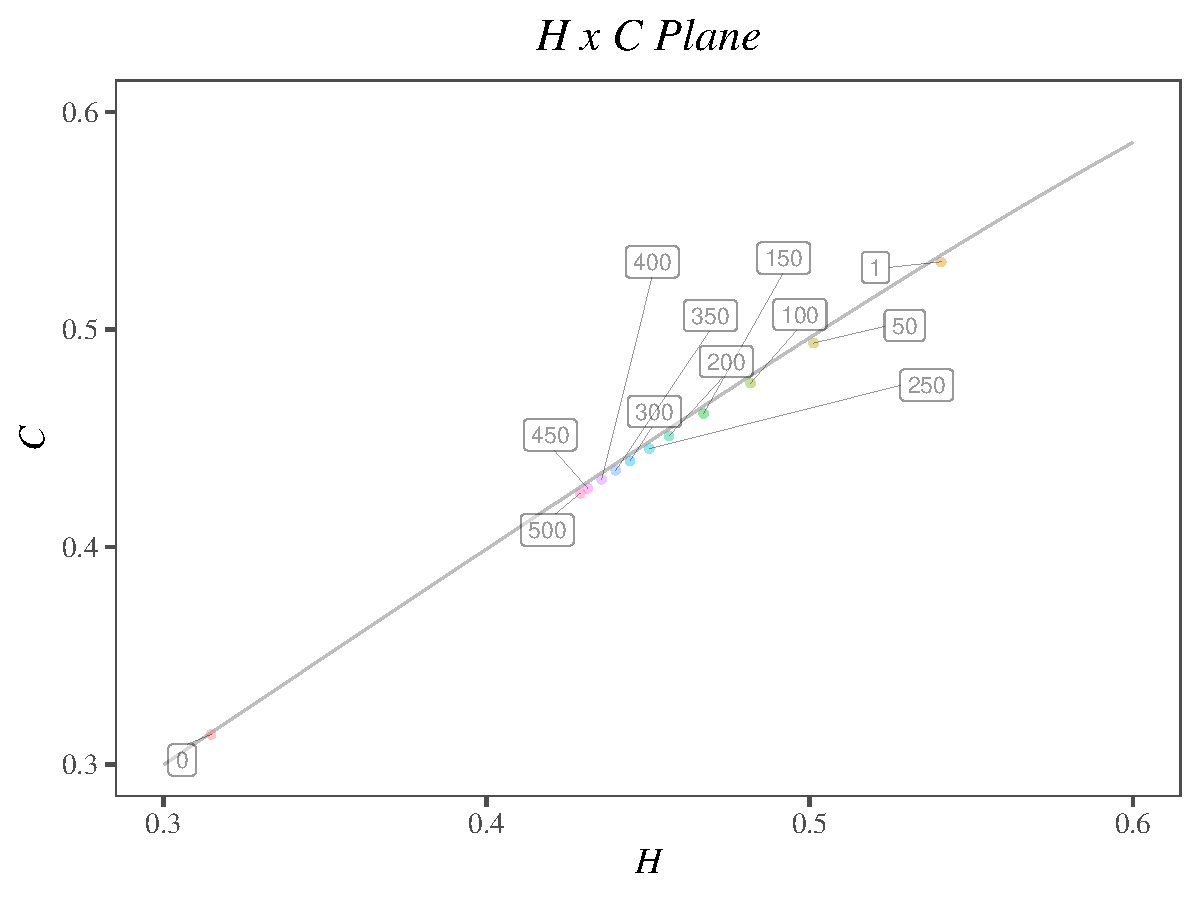
\includegraphics[width=.6\linewidth]{Figures/waves1.pdf}
 	\captionof{figure}{Modifications to the $H \times C$ Plane features by adding different multiplicative noises.}
 	\label{Fig:TestSpeckleHC}
% \end{figure}
\end{minipage}
\end{tcolorbox}

\vskip3em\begin{tcolorbox}[colback=red!5!white,colframe=red!75!black,title=Comment \#13]
	What can we conclude on all the presented weight techniques? 
	What to use at the end from a thematic point of view?
\end{tcolorbox} 

First, as explained in the response of Comment \#7, the original Bandt-Pompe transformation does not consider the amplitude of the signal; hence, it is not appropriate to capture the scattering properties of SAR imagery, as we can observe in the classification results. Moreover, we also observed that using traditional weighting techniques to encode the amplitude information to the histogram of ordinal patterns did not perform well. 
Our proposal considers not only the ordinal patterns but the first-order transitions among them. By encoding the amplitude information in this model, we observed that the spatial correlation of the images was preserved and that we could properly capture this structure. 
We also observed that the classification results are comparable to techniques that use a much larger number of features. 
Thus, our proposal presents highly competitive results. 
Many applications can benefit from such a discriminant approach, such as texture segmentation and border detection.

We added a paragraph with the evaluation of the results obtained by these techniques at the end of subsection III-C:
% In experiments carried out with homogeneous textures,
% we found that for the analyzed data set, the weighting techniques in the histogram of ordinal patterns cannot fully describe different samples of SAR textures.
% The best results, in general, are obtained by WATG, since the amplitude is no longer weighed by the pattern histogram, but by the transition graph, giving greater importance to transitions with wide variations in intensity.

\vspace{.4cm}
\begin{tcolorbox}[colback=white,colframe=black,title=Change \#13]
	
	
	"Table I shows that, among the methods of weighting ordinal patterns, FGPE produced the worst results: $\text{AA} = \SI{76.7}{\percent}$, $\text{F1-score}_\mu = \SI{86.8}{\percent}$, and $\text{F1-score}_M = \SI{71.1}{\percent}$.
    %
    WPE also produced a low F1-score, but it produced consistently better results in the other metrics, presenting $\text{AA} = \SI{93.3}{\percent}$.
    %
    AAPE achieved one of the best F1-score results: $\text{AA} = \SI{83.3}{\percent}$, $\text{F1-score}_\mu = \SI{94.7}{\percent}$, and $\text{F1-score}_M = \SI{89.6}{\percent}$.
    %
    WATG, considering the transition graph of ordinal patterns, can better describe the textures presented, as it achieves the best performance achievable in all metrics: \SI{100}{\percent}."	
\end{tcolorbox}

\section{Reviewer \#3}

\vskip3em\begin{tcolorbox}[colback=red!5!white,colframe=red!75!black,title=Comment \#1]
	The authors would better provide a clear motivation of proposed method in abstract. Why the Bandt-Peano symbolization is employed in this paper. The readers can be then interested in this work
\end{tcolorbox} 

We reformulated the abstract and also the introduction to better motivate our proposal. The abstract now reads:

\begin{tcolorbox}[colback=white,colframe=black,title=Change \#1]
	
	“The use of Bandt-Pompe probability distributions and descriptors of Information Theory has been presenting satisfactory results with low computational cost in the time series analysis literature~\cite{Aquino2017Characterization, Rosso2016Signatures, Schieber2016network}.
	However, these tools have limitations when applied to data without time dependency.
	Given this context, we present a newly proposed technique for texture analysis and classification based on the Bandt-Pompe symbolization for SAR data.
	It consists of
	(i)~linearize a \mbox{2-D} patch of the image using the Hilbert-Peano curve,
	(ii)~build an Ordinal Pattern Transition Graph that considers the data amplitude encoded into the weight of the edges;
	(iii)~obtain a probability distribution function derived from this graph;
	(iv)~compute Information Theory descriptors (Permutation Entropy and Statistical Complexity) from this distribution and use them as features to feed a classifier.
	The ordinal pattern graph we propose considers that the weight of the edges is related to the absolute difference of observations, which encodes the information about the data amplitude. 
	This modification takes into account the scattering properties of the target and leads to the characterization of several types of textures.
	Experiments with data from Munich urban areas, Guatemala forest regions and Cape Canaveral ocean samples show the effectiveness of our technique in homogeneous areas, which achieves satisfactory levels of separability.
	The two descriptors chosen in this work are easy and quick to calculate and are used as input for a k-nearest neighbor classifier.
	Experiments show that this technique presents results similar to state-of-the-art techniques that employ a much larger number of features and, consequently, require a higher computational cost.”
\end{tcolorbox}

\vskip3em\begin{tcolorbox}[colback=red!5!white,colframe=red!75!black,title=Comment \#2]
	The authors would better polish the English description. The current version is really not up to scratch of a top-tier journal.
\end{tcolorbox} 

Thanks for the recommendation, we performed a careful proof-reading to the manuscript.

\vskip3em\begin{tcolorbox}[colback=red!5!white,colframe=red!75!black,title=Comment \#3]
	In the first page, there are more than 10 paragraphs. The similar structure can be found in the remaining sections. The authors would better organize this paper in the formalism of scientific paper.
\end{tcolorbox} 

\begin{tcolorbox}[colback=white,colframe=black,title=Change \#3]
	The article was fully revised to improve its organization and clarity.
\end{tcolorbox}

\vskip3em\begin{tcolorbox}[colback=red!5!white,colframe=red!75!black,title=Comment \#4]
	The recent development of texture analysis and classification in SAR images are very short. The authors would better discuss much more related studies in literature. Both the handcrafted features and the learned representations should be reviewed.
\end{tcolorbox} 
We improve the literature review adding the following text to Section I:
\begin{tcolorbox}[colback=white,colframe=black,title=Change \#4]
	
    ``Surface classification and land use are among the most important applications of the Synthetic Aperture Radar (SAR) image~\cite{Pottier2004Unsupervised}.
    In recent years, handcrafted features and representation learning (supervised and unsupervised) algorithms have been proposed~\cite{han2020unsupervised, huang2020classification, xie2020polsar}.
    Algorithms of the unsupervised generative adversarial network (GAN) have revolutionized the classification of SAR images, improving performance in small sample problems, and helping the interpretability of such data~\cite{liu2019task}.
    Among the supervised algorithms, support vector machine (SVM)~\cite{sukawattanavijit2017ga}, random forest (RF)~\cite{mcnairn2014early}, and neural network (NN)~\cite{lin2017deep} have been frequently used in remote sensing.
    The Principle Component Analysis (PCA)~\cite{ressel2015neural}, autoencoder~\cite{wang2019classification} and the Boltzmann machine~\cite{qin2017object} can to extract non-local resources and classify non-labeled PolSAR pixels using an unsupervised approach.
    However, methods such as graph-based semi-supervised deep learning algorithms~\cite{bi2018graph} can improve classification accuracy in problems with few labeled samples.
    
    Handcrafted features in SAR textures can be studied following two complementary approaches, namely analyzing the marginal properties of the data (first-order statistics), and observing their spatial structure~\cite{Yue2020Gaussian, numbisi2018multi}.
    In this work, we focus on the second approach, which has been showing relevant results using techniques from the image processing literature, such as co-occurrence matrices and Haralick's descriptors~\cite{yu2019detection}.
    Through the GLCM we can extract features that reflect statistical relationships of the pixel intensity values.
    On the other hand, Haralick's descriptors can capture information on intensity and amplitude based on global statistics of SAR images.
    Radford et al.~\cite{radford2018geological} used textural information derived from gray-level co-occurrence matrices (GLCM), along with Random Forests, for geological mapping of remote and inaccessible localities; the authors obtained a classification accuracy of $\approx\SI{90}{\percent}$, even when using limited training data ($\approx\SI{0.15}{\percent}$ of the total data). 
    Hagensieker and Waske~\cite{hagensieker2018evaluation} evaluated the synergistic contribution of multi-temporal L-, C-, and X-band data to tropical land cover mapping, comparing classification outcomes of ALOS-2~\cite{kankaku2013alos}, RADARSAT-2~\cite{morena2004introduction}, and TerraSAR-X~\cite{breit2009terrasar} datasets for a study site in the Brazilian Amazon using a wrapper approach. 
    The wrapper utilizes the gray-level co-occurrence matrix texture information and a  Random Forest classifier to estimate scene importance. 	
    Storie~\cite{storie2018urban} proposed an open-source workflow for detecting and delineating the urban-rural boundary using Sentinel-1a SAR data.
    The author used a combination of GLCM information and a k-means classifier to produce a three-category map that distinguishes urban from rural areas. In higher 
\end{tcolorbox}
\begin{tcolorbox}[colback=white,colframe=black,title=Change \#4]
    resolution image classification activities, it is necessary to obtain more granular information from the data by extracting local characteristics of the data, such as scale and orientation.
    In this scenario, techniques such as Fourier power spectrum~\cite{Florindo2012Fractal}, random fields~\cite{zhu2016antarctic}, Gabor filter~\cite{dumitru2014information} and wavelet transform~\cite{akbarizadeh2012new} are usually applied.''
\end{tcolorbox}


\vskip3em\begin{tcolorbox}[colback=red!5!white,colframe=red!75!black,title=Comment \#5]
	In Section II, the motivation of proposed strategy is not described clearly. Why the Bandt-Peano symbolization has been employed. The author would better provide a clear explanations.
\end{tcolorbox} 

 We rephrase the Introduction to improve the motivation and the methodology of our proposal:

\begin{tcolorbox}[colback=white,colframe=black,title=Change \#5]
   
    
    ``The following question guides us:
\begin{quote}
What is the best representation of a texture patch that allows extracting expressive Information Theory descriptors to characterize textures in the presence of speckle?
\end{quote}
We verified that both the histogram of Bandt-Pompe ordinal patterns and classical transition graphs do not convey enough information for suitable applications as, for instance, classification.

Henceforth, we propose the Weighted Amplitude Transition Graph (WATG).
This graph incorporates the absolute difference among observations as weights of the edges between nodes transitions.
Such weights take part in the computation of the probabilities and, thus, influence both Entropy and Statistical Complexity.

This work's main contribution is the proposal of a new representation of SAR textures, which allows a low-dimensional characterization useful for, among other applications, their classification.
We compare its performance with the classical histograms of Bandt-Pompe ordinal patterns and the regular transition graph.
Since the proposed approach has a low computational cost, the results obtained suggest that this technique has good potential in other applications, such as texture segmentation tools of SAR images.''
\end{tcolorbox}


\vskip3em\begin{tcolorbox}[colback=red!5!white,colframe=red!75!black,title=Comment \#6]
	The organization of this paper is a bit chaos. What is the relation between Section II-D and Section III. In my opinion, Section III can be merged into Section II.
\end{tcolorbox} 

\begin{tcolorbox}[colback=white,colframe=black,title=Change \#6]
	As suggested, we merged sections III and II. We followed the IMRAD\footnote{https://en.wikipedia.org/wiki/IMRAD} scientific paper organization to provide a more familiar text organiztion to the reader.
\end{tcolorbox}

\vskip3em\begin{tcolorbox}[colback=red!5!white,colframe=red!75!black,title=Comment \#7]
	The experiments on Quantitative Evaluation is very limited. In my opinion, they are not convincing. The authors would better provide much more comparative studies with state-of-the-art methods. The comparisons with deep learned representations may be much more convincing than handcrafted features.
\end{tcolorbox} 

We enhanced the experimental part with samples of pasture/culture.
The problem presented consists of $200$ samples, and as presented in section II-H, we randomly split the samples in training (\SI{85}{\percent}) and test (\SI{15}{\percent }) sets.
We used the first set to train a $k$-nearest neighbor classifier algorithm with tenfold cross-validation.

Our technique showed to be simple, requires only the extraction of two features, and reaches top-class performance. We chose not to compare it to approaches that are hard to train (the number of hyperparameters is typically high compared to the data size), prone to overfitting, and lack interpretability.

\vspace{.4cm}
\begin{tcolorbox}[colback=white,colframe=black,title=Change \#7]
	To improve the baseline used, we added three more techniques:
    Histogram of oriented gradients (HOG)~\cite{dalal2005histograms},
    Speeded-Up Robust Features (SURF)~\cite{bay2006surf}, and
    Short Time Fourier Transform (STFT)~\cite{portnoff1980time} with Speeded-Up Robust Features (SURF).
\end{tcolorbox}

\bibliographystyle{IEEEtran}
\bibliography{AbbrevRefs}

\end{document}

